\textbf{Motivation.} End-to-end encryption is an encryption such that the only communicating parties
are able to decrypt the data.
It means that even system administrators are not able to decrypt the messages transmitted between parties
via their communication channel.
End-to-enc encryption can be reached via numerous approaches.
Generally, there are two ways to implement E2E encryption
\begin{itemize}
    \item Sharing public key to be used in decryption of the secret message, then encryption is done by the
    public key's owner, so-called asymmetric encryption.
    For example, RSA algorithm.
    \item Asymmetric key exchange, where parties firstly exchanging the keys, then symmetrically encrypting
    the transferred data.
    For instance, Diffie--Hellman key exchange and AES256 encryption using common secret.
\end{itemize}
The most important aspect here is to securely store the secrets on the user's client application.
Due to storage issues, it doesn't make sense to implement E2E encryption for web
and desktop clients, like it is done in nowadays popular Telegram Messenger
[\cite{job2015modified,suvsanka2017security,lee2017security}].
Telegram uses the huge and heavy \texttt{MTProto 2.0} cryptographic protocol, based on DH key exchange and further AES256
symmetric encryption.
According to the project concerns, the E2E encryption via Diffie--Hellman key exchange and AES256
to be considered and implemented, the next section is about.

\textbf{Diffie–-Hellman key exchange.} Diffie--Hellman protocol is a method of asymmetric exchange
of the cryptographic keys for a group of two or more participants,
developed in 1976 by cryptographers Ralph Merkle, Whitfield Diffie and Martin Hellman.
In contrast to symmetric key exchange, the Diffie–-Hellman protocol eliminates the direct transfer of the shared secret.
between participants, each participant computes a shared secret with its own private-public key pair.
The Diffie–-Hellman protocol is based on a one-way function of the form

\[
    A = G ^ a \bmod P,
\]

where $A$ is the user's public key, $a$ is the user's private key, $P$ is modulus, which is at least 2048 bit prime,
$G$ is primitive root modulo $P$.

Thus, the safety of the Diffie--Hellman protocol is based on the discrete logarithm problem, which is unsolvable
in polynomial time if the constants $G$ and $P$ are chosen correctly.
Graphically, the essence of the Diffie–-Hellman protocol can be expressed through the analogy with mixing paints,
as shown in image below
\begin{figure}[H]
    \centering
    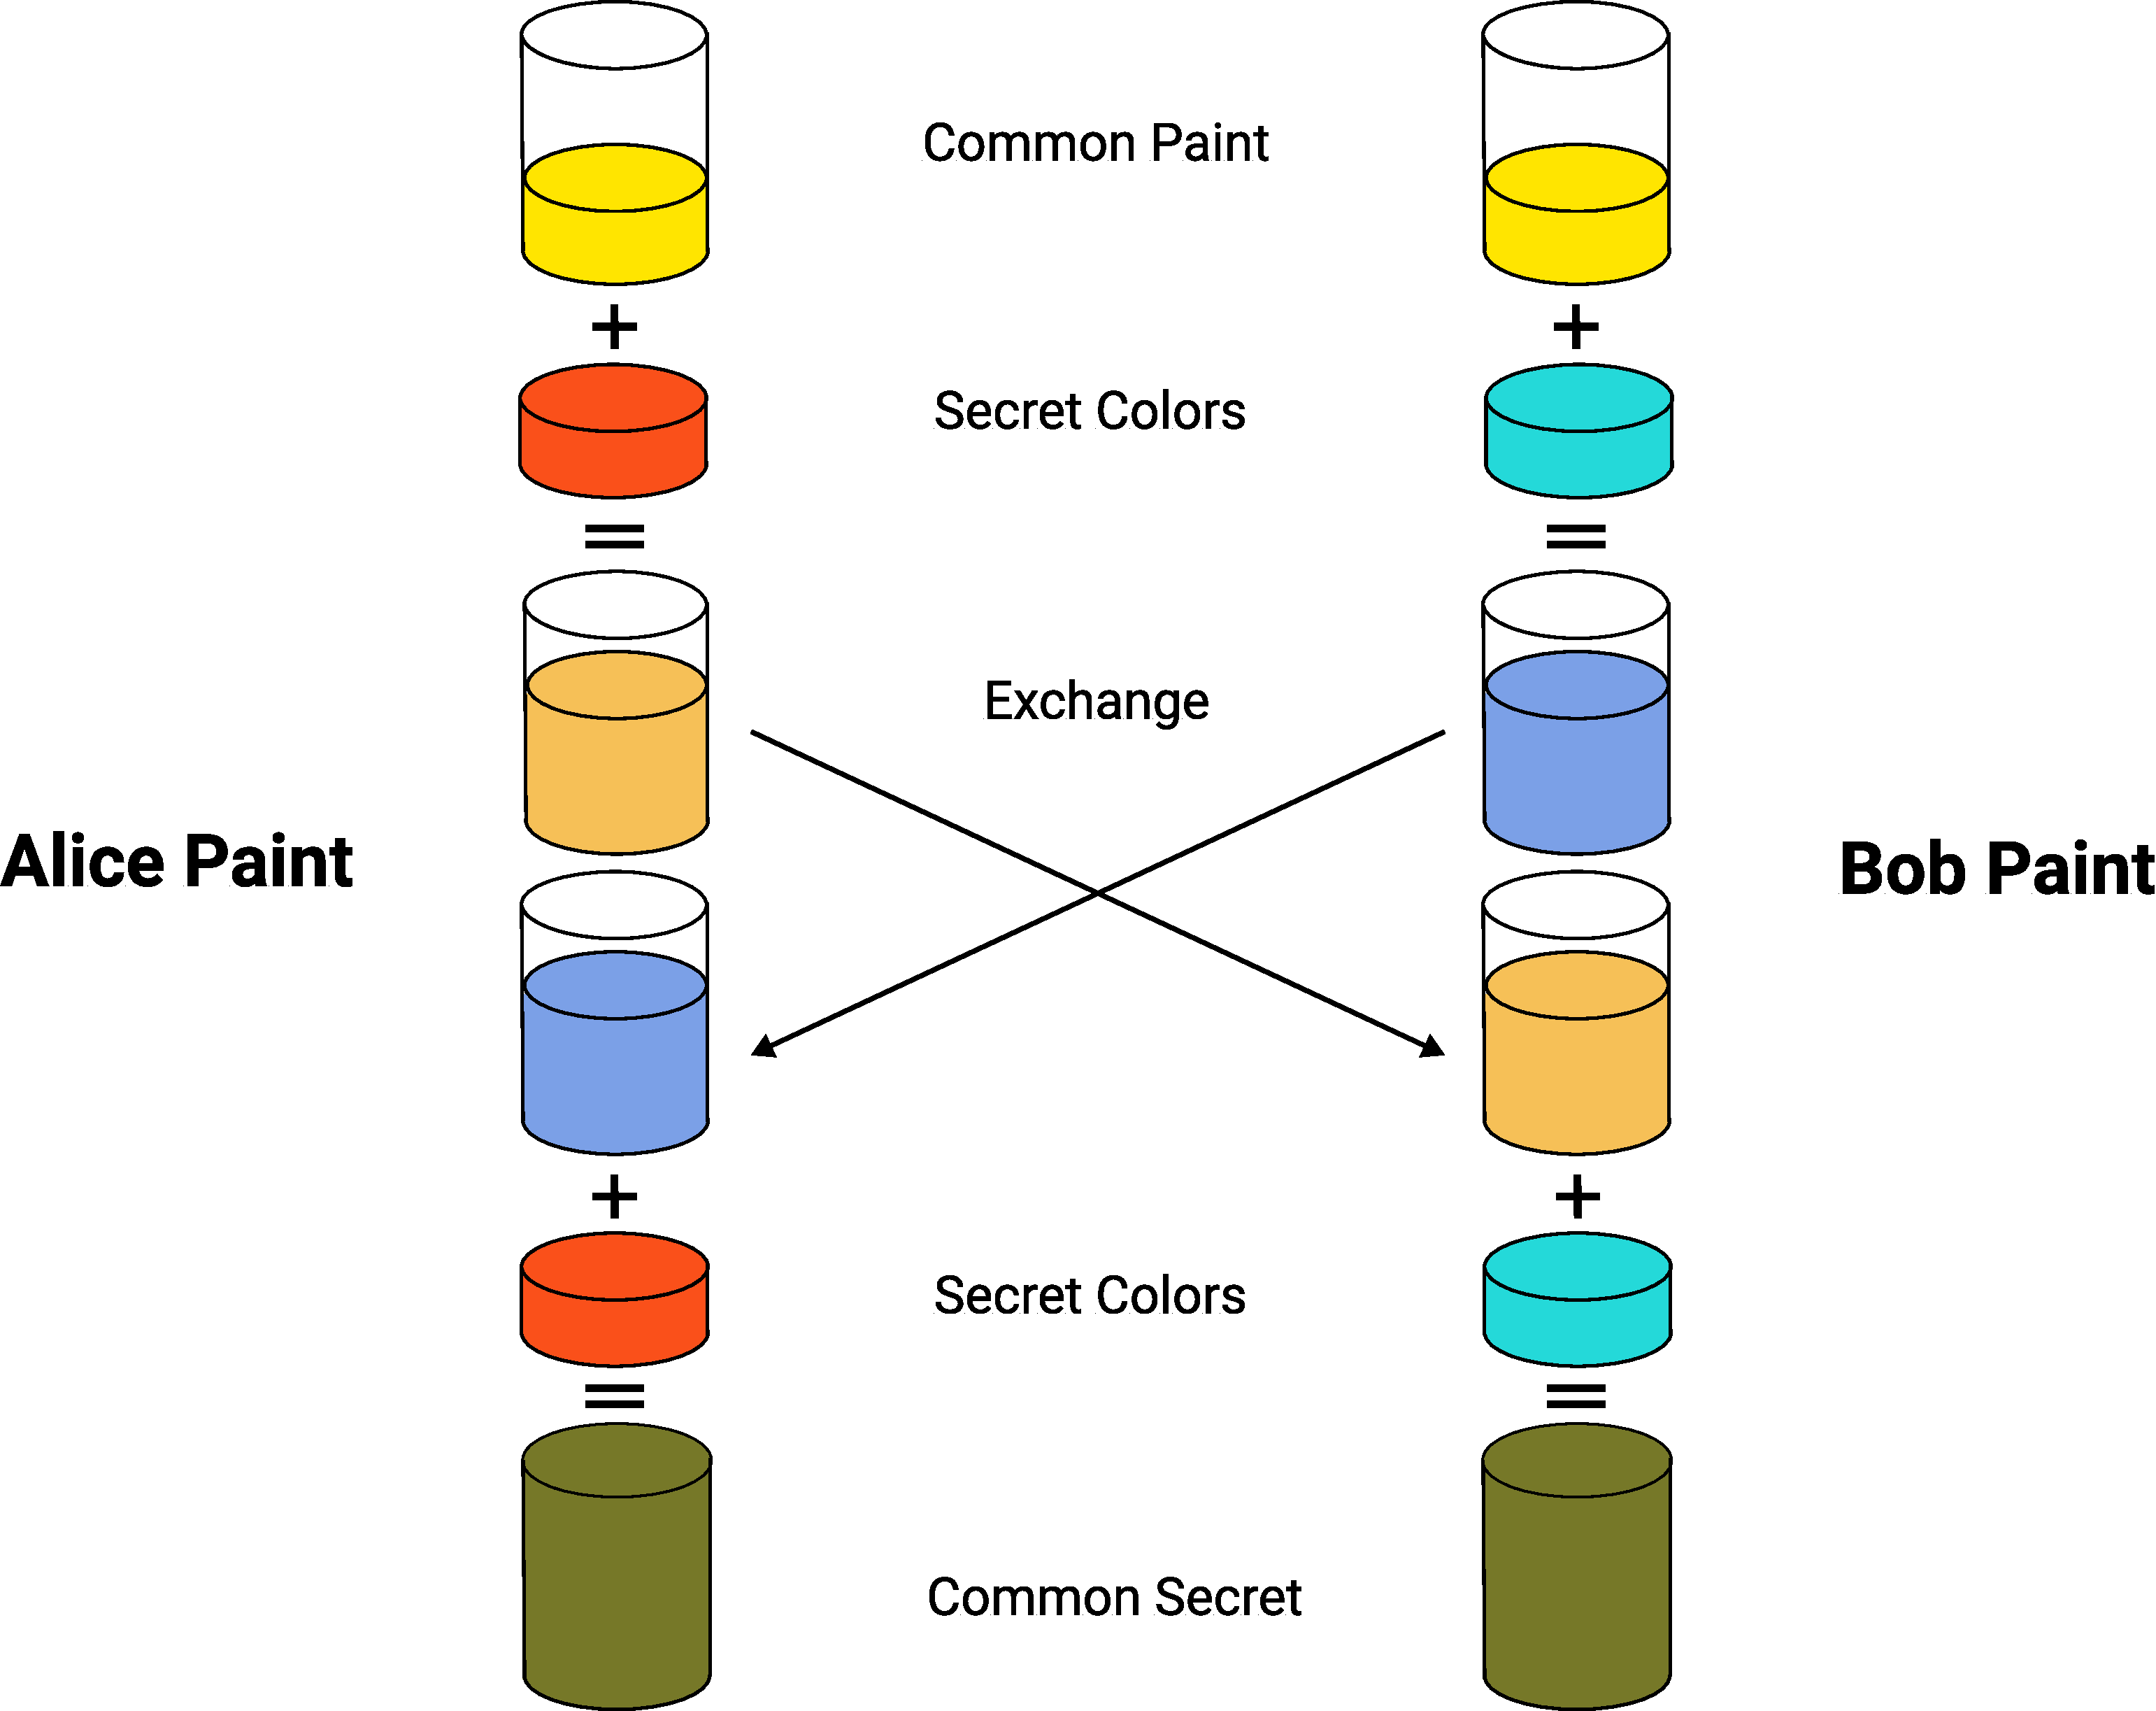
\includegraphics[width=1\textwidth]{Pictures/07_Diffie-Hellman_keyexchange_concept_diagram}
    \caption{Diffie–-Hellman key exchange concept diagram.
    Source: \href{https://en.wikipedia.org/wiki/Diffie-Hellman_key_exchange}{Wikipedia}.}\label{fig:figure4}
\end{figure}
In contrast to the Diffie–-Hellman based on discrete logarithm problem, there is an elliptic curve diffie hellman
key exchange, which based on the elliptic curve discrete logarithm problem.
Although, the idea is quite same, the difference only in that elliptic curve Diffie–-Hellman ensures the same safety
as discrete logarithm Diffie–-Hellman with lower value of the prime modulus $P$.
For instance, 521 bit modulus used in elliptic curve Diffie–-Hellman is equally safe as 2048 bit modulus in
discrete logarithm Diffie–-Hellman.
To summarize, the flow of Diffie–-Hellman key exchange is as follows
\begin{enumerate}
    \item Given 2048 bits prime modulus $P$ and generator $G$, such that $G$ is primitive root modulo $P$.
    \item Alice chooses her secret $a$.
    \item Alice sends to Bob her public key $A = G^a \bmod P$.
    \item Bob chooses his secret $b$.
    \item Bob sends to Alice his public key $B = G^b \bmod P$.
    \item Alice computes common secret $s = B^a \bmod P$.
    \item Bob computes common secret $s = A^b \bmod P$.
    \item Alice and Bob have arrived to the same value
    \begin{eqnarray*}
        A^b \bmod P = G^{ab} \bmod P \\
        B^a \bmod P = G^{ba} \bmod P
    \end{eqnarray*}
\end{enumerate}

\textbf{Implementation.} Although, the idea of DH key exchange looks quite simple, some remarks on the concrete
implementation should be added.
Firstly, it is necessary to implement the mechanism of key exchange request between two or more parties.
As it discussed above, each user has his own private-public keys pair, so in order to perform request between parties,
it should be implemented dedicate REST API endpoint, for instance the POST one \texttt{api/key-exchange-requests} which
takes the body of the form
\begin{spverbatim}
{
    "requestedUserId": "3fa85f64-5717-4562-b3fc-2c963f66afa6",
    "publicKey": "RUNLMSAAAAC2lkqYcTGhutQPxcjvoqUELKoy0"
}
\end{spverbatim}
So, request sender generates on the client side a key pair, keeps private on in the file system and shares the public
in request to receiver.
Therefore, the second party has received the key exchange request.
In order to display all the key exchange requests awaiting the confirmation of decline decisions, it is worth to implement
another REST endpoint such that GET \texttt{api/key-exchange-requests}, so that requested party will have the list of
requests to proceed.
This endpoint may return the data structure like follows
\begin{spverbatim}
{
    "keyExchangeRequests": [
        {
            "requestId": "81d314c1-913f-4686-827e-ef2a65ccc370",
            "senderId": "3fa85f64-5717-4562-b3fc-2c963f66afa6",
            "senderPublicKey": "RUNLMSAAAAC2lkqYcTGhutQPxcjvoqUELKoy0"
        }
    ],
    "message": "SUCCESS",
    "success": true
}
\end{spverbatim}
Finally, requested party should be able to confirm or decline the key exchange request, the DELETE endpoint
\texttt{api/key-exchange-requests} should be implemented then.
The server is able to fetch the request thanks to the body endpoint takes
\begin{spverbatim}
{
    "requestId": "3fa85f64-5717-4562-b3fc-2c963f66afa6",
    "confirmed": true,
    "publicKey": "string"
}
\end{spverbatim}
Therefore, an identifier of awaiting request is passed to the server among with boolean value
indicating the confirmation.
Under the roof of this operation are also generation of private-public keys pair for the requested party and
generation of common secret stored in client's file system.
As result, the initial request sender receives a public key as confirmation from requested party.
Requested side may get all his public keys via the REST API using GET \texttt{api/public-keys}
\begin{spverbatim}
{
    "publicKeys": [
        {
            "partnerId": "ae9e10a4-0c7e-4911-8450-4139d4a114a7",
            "partnerPublicKey": "RUNLMSAAAAAbc49wfaZ+QF9J2cu1S66bkp0"
        }
    ],
    "message": "SUCCESS",
    "success": true
}
\end{spverbatim}
Now requested participant is able to derive the common secret.
In order to provide an example, a simple command line interface is implemented.
We have used an Elliptic Curve Diffie–-Hellman implementation \texttt{ECDiffieHellmanCng Class} from the namespace
\texttt{System.Security.Cryptography} of the .NET base class library.
The \texttt{P-256} curve is used.

More precisely, the following CLI commands are implemented
\begin{itemize}
    \item \texttt{MangoAPI.DiffieHellmanConsole login SENDER\_EMAIL SENDER\_PASSWORD}
    \item \texttt{MangoAPI.DiffieHellmanConsole key-exchange RECEIVER\_ID}
    \item \texttt{MangoAPI.DiffieHellmanConsole key-exchange-requests}
    \item \texttt{MangoAPI.DiffieHellmanConsole confirm-key-exchange REQUEST\_ID}
    \item \texttt{MangoAPI.DiffieHellmanConsole print-public-keys}
    \item \texttt{MangoAPI.DiffieHellmanConsole create-common-secret RECEIVER\_ID}
\end{itemize}
Commands are self-explanatory, therefore we skip the detailed documentation on them.
An example of console output straightforward
\begin{figure}[H]
    \centering
    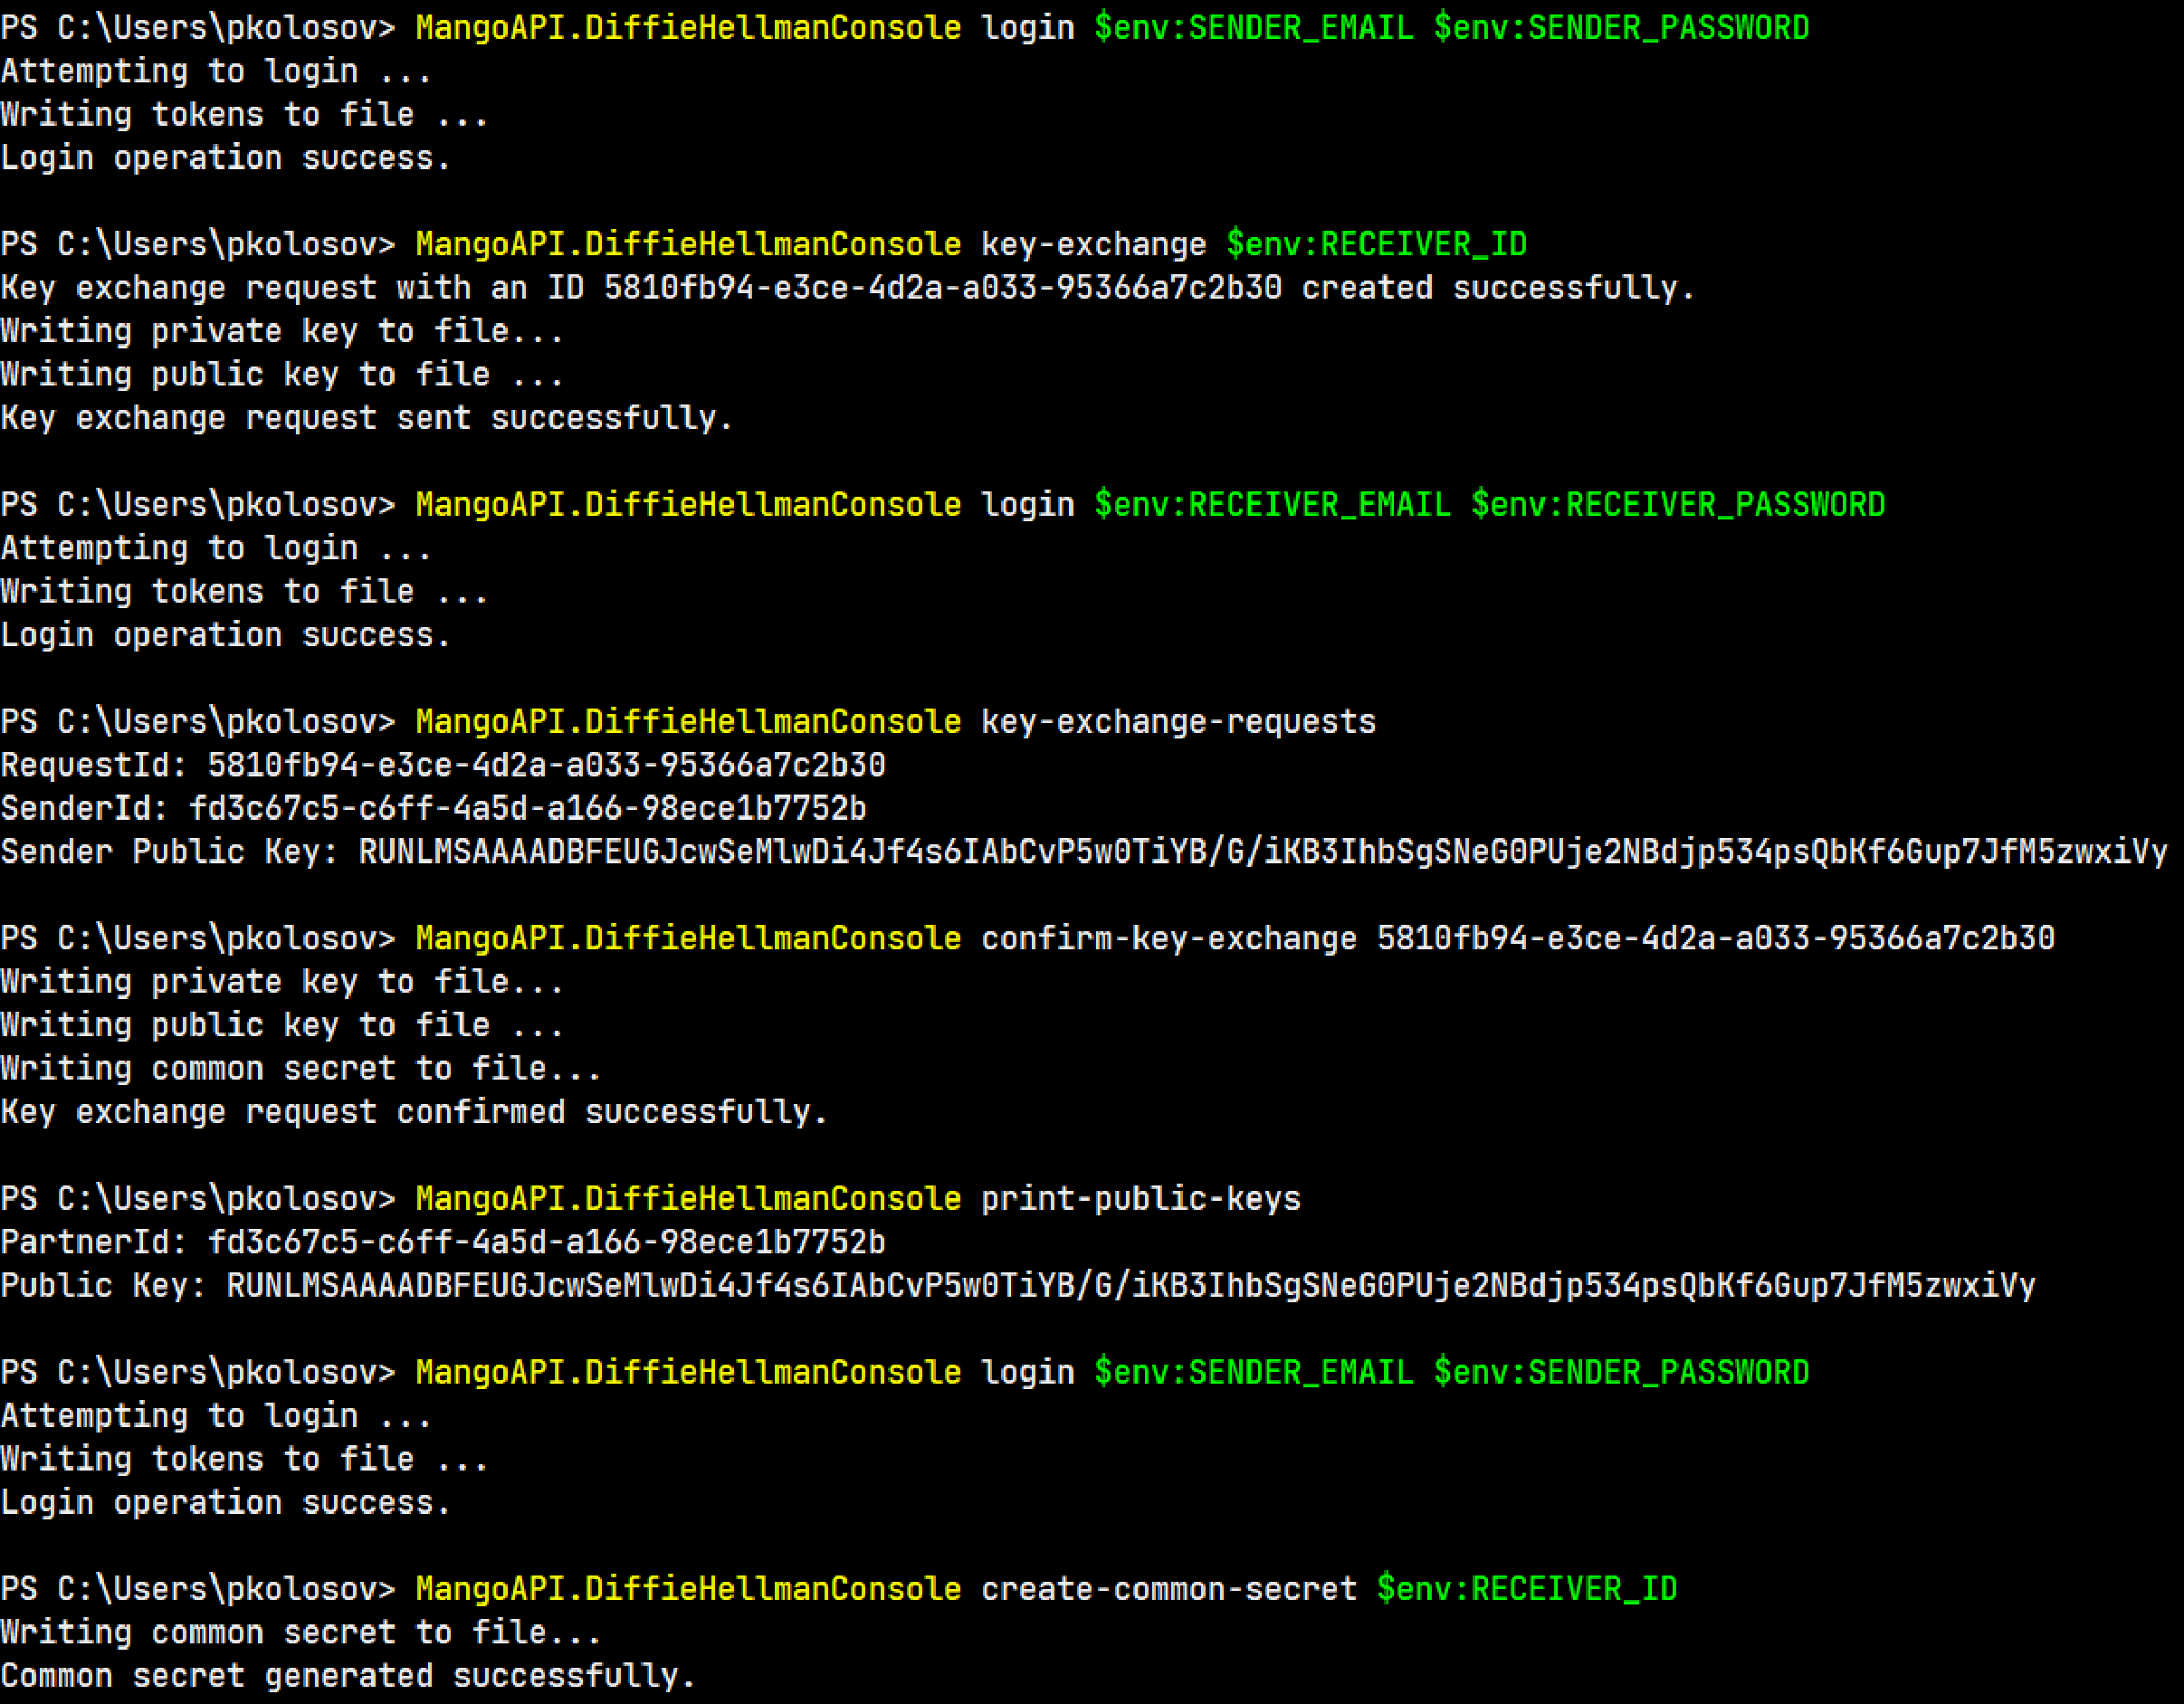
\includegraphics[width=1\textwidth]{Pictures/08_Diffie-Hellman_console_output}
    \caption{Diffie–-Hellman key exchange console output.}\label{fig:figure7}
\end{figure}
Finally, both test accounts reached the same common secret.
In order to work with our implementation of the ECDH key exchange, the user is obligated to register an account
at \href{https://messenger-mango.herokuapp.com}{https://messenger-mango.herokuapp.com}.